\documentclass{article}

\usepackage[utf8]{inputenc}
\usepackage{geometry}
\usepackage{graphicx}


\usepackage{hyperref}

\usepackage{float}

\delimitershortfall-1sp
\newcommand\abs[1]{\left|#1\right|}


\title{Visualización de Datos MedioAmbientales de Castilla y León}
\author{Sergio García Prado}


\begin{document}

	\begin{titlepage}
		\centering
		{\scshape\LARGE Universidad de Valladolid \par}
		\vspace{1cm}
		{\scshape\Large Diseño y Evaluación de Sistemas Interactivos\par}
		\vspace{1.5cm}
		{\huge\bfseries Análisis y Visualización de Datos MedioAmbientales de Castilla y León\par}
		\vspace{2cm}
		{\Large\itshape Sergio García Prado\par}

		\vfill
		Seguimiento del trabajo en: \par
		\href{https://github.com/garciparedes/DatosMedioambientalesCYL}{github.com/garciparedes/DatosMedioambientalesCYL}
		\vfill


		% Bottom of the page
		{\large \today\par}
	\end{titlepage}



	\newpage
		\tableofcontents
	\newpage


	\section{Introducción}

		\subsection{Motivación}

			\paragraph{}
			La visualización que se va a realizar consiste en la representación gráfica de datos medioambientales de la Comunidad Autónoma de Castilla y León. El objetivo de la práctica es descubrir aspectos poco obvios o destacar algo importante del conjunto de datos asignados.

		\subsection{Objetivos}

			\paragraph{}
			La representación gráfica que se va a realizar pretende mostrar el flujo energético en Castilla y León durante los últimos años. 
			Además una vez se pueda visualizar la implementación se pretenden obtener conclusiones sobre el impacto que ha tenido el cierre de la Centrar Nuclear de Santa María de Garoña (Burgos) en el año 2012 y representar cómo ha solventado la región ese déficit energético (si es que lo ha hecho). También se pretende analizar si este suceso está ha afectado al consumo energético en la zona.

	\section{Análisis de los datos}

		\subsection{Descripción}
			\paragraph{}
			La Junta de Castilla y León suministra conjuntos de datos referentes a la comunidad autónoma. Para esta práctica se nos han asignado los datos medioambientales.

		\subsection{Adquicisión}
			\paragraph{}
			Los datos han sido obtenidos a partir de la iniciativa de Datos Abiertos de la Junta de Castilla y León.

			\paragraph{}
			El concepto "datos abiertos" es una filosofía y práctica que persigue que determinados tipos de datos estén disponibles de forma libre para todo el mundo, sin restricciones de derechos de autor, de patentes o de otros mecanismos de control. Tiene una ética similar a otros movimientos y comunidades abiertos, como el software libre, el código abierto y el acceso libre.

			\paragraph{}
			Los datos han sido obtenidos a partir del siguiente enlace: \href{http://www.datosabiertos.jcyl.es/web/jcyl/set/es/mediciones/indicadoresambientales/1284227444931}{www.datosabiertos.jcyl.es/...}

			\paragraph{}
			Una vez hemos obtenido los datos procederemos a realizar el análisis de los mismos.

		\subsection{Estructura de los datos}

			\paragraph{}
			Los datos que vamos a manejar se encuentran en fichero con formato CSV (un tipo de documento en formato abierto sencillo para representar datos en forma de tabla, en las que las columnas se separan por comas (o punto y coma) y las filas por saltos de línea.), el cual a pesar de tener una estructura eficiente para ser manejado por máquinas, complica la lectura y extracción de información para los humanos. Además la cantidad de información contenida en este grande (más de 5000 elementos).

			\paragraph{}
			A pesar de estas dificultades, fijándonos en la cabecera del fichero, la cual nos da información de la estructura de los mismo, podemos conocer lo campos nos encontraremos en cada una de las filas que contiene:

			\begin{itemize}

				\item {\bf Indicador } Contiene información sobre a lo que se refiere el dato. Representa una variable de tipo cualitativo nominal. Tras realizar una extracción de datos, hemos obtenido que hay 49 indicadores distintos. Debido a que la cantidad es numerosa habrá que tratar de seleccionar los que más se adecuen a lo que queremos mostrar debido a que mostrar demasiada información de manera inadecuada dificulta la visión de lo que se pretende representar.

				\item {\bf Provincia } Provincia a la que está referida la información. Este campo es de tipo cualitativo nominal. Se refiere a la segmentación territorial de la comunidad autónoma. Como sabemos, Castilla y León está dividida en 9 provincias. Conviene señalar que hay indicadores que no poseen información para todas las provincias, como es el caso del "Tráfico aéreo de pasajeros", que suponemos que restringe la información a las provincias que disponen de aeropuerto ya que el resto tendrían valor 0 y no tiene sentido indicarlo. Este hecho es algo a tener en cuenta cuando representemos la información.

				\item {\bf Fecha Validez } Fecha hasta la cual el dato se consideraba como actual. Representa una variable cuantitativa debido a que es una variable temporal. A pesar de ello toma únicamente valores discretos (años). Esto es algo a tener en consideración cuando determinemos la manera en que será representado.

				\item {\bf Valor } Valor que toma el dato respecto de su unidad.  Representa una variable cuantitativa de tipo continuo. Este campo es el que contiene la "información valiosa", ya que es lo que se utilizará como medida para compararla con los demás. Se representa en forma de número racional positivo.

				\item {\bf Unidad } Este campo nos proporciona la unidad de medida del dato, lo cual es algo muy importante a la hora de mostrar información ya que siempre se deben señalar tanto la unidad de medida como la escala a la que corresponde la información representada.

				\item {\bf Frecuencia } Este campo representa la periodicidad con la que se ha obtenido el dato. La mayoría de los datos se han obtenido anualmente, aunque también existen algunos que se han obtenido bianualmente, como es el caso de los "Espacios Naturales".

			\end{itemize}

		\subsection{Calidad}

			\paragraph{}
			A mi juicio la calidad de los datos es buena a pesar de que existen algunos puntos  mejorables.

			\paragraph{}
			Me llama la atención la columna de "meses" que, entiendo que está ahí porque es necesario espedificar la unidad de medida de la frecuencia, pero creo que se debería haber indicado en la cabecera del fichero. Además también he encontrado valores atípicos en algunos datos, posiblemente producidos por un error en las mediciones o al transcribirlo al documento.

		\subsection{Selección de datos}

			\paragraph{}
			Ahora determinaremos los datos que se utilizarán para la visualización. Como se dijo al principio del informe, el objetivo de la visualización será visualizar cómo a repercutido el cierre de la central nuclear en la región. Para ello nos vamos a apoyar en los siguientes indicadores:

			\begin{itemize}
				\item Producción de energía con carbón
				\item Producción de energía eólica
				\item Producción de energía hidráulica
				\item Producción de energía nuclear
				\item Producción de energía primaria
				\item Producción energía solar en Castilla y León
				\item Consumo de energía final
				\item Consumo de energía del sector del transporte
				\item Consumo de energía del sector
				\item Consumo doméstico de electricidad
				\item Consumo doméstico de gas natural
				\item Consumo doméstico de G.L.P.
				\item Consumo doméstico de productos petrolíferos
			\end{itemize}

			\paragraph{}
			De cada uno de estos indicadores se pretenten utilizar tanto la información de todas las provincias como fechas de validez.

		\subsection{Transformaciones}

			\paragraph{}
			Para simplificar la visualización realizaremos varias transformaciones en los datos:

			\paragraph{}
			Fusionaremos estos indicadores en uno nuevo que denominaremos "Producción de energía final" cuyo valor será el sumatorio de todos los métodos de producción (Carbón, Eólica, Hidráulica, Nuclear, Primaria y Solar). La unidad de medida de todos ellos es "Toneladas Equivalentes de Petróleo" por lo cual no habrá que realizar ningún cambio de unidad para poder fusionarlos.

			\paragraph{}
			Para clarificar el tipo de energía que se utiliza se ha decidido crear dos otros dos nuevos indicadores denominados "Producción de Energía Renovable" y "Producción de Energía No Renovable" que se formarán a partir del sumatorio de sus respectivos métodos de energía.

			\paragraph{}
			 También fusionaremos los indicadores relacionados con el consumo doméstico en uno nuevo que  denominaremos  "Consumo Doméstico" cuyo valor será el sumatorio de estos (Electricidad, Gas Natural, G.L.P. y Productos Petrolíferos). En este caso la información no tiene la misma unidad de medida para todos ellos, por lo que habrá que adaptar cada uno de ellos a la misma (Toneladas Equivalentes de Petróleo) para luego crear el nuevo indicador a partir de estos. El motivo de convertirlos en Toneladas Equivalentes de Petróleo nos servirá para luego compararlos con los indicadores de  producción energética.


	\section{Planificación de la información}

		\subsection{Propósito de la visualización}

			\paragraph{}
			El proyecto de visualización se va a enfocar en el sector energético. El objetivo de la visualización es mostrar la relación entre la producción y el consumo energético de la comunidad autónoma. Además de mostrar la proporción tanto de los diferentes métodos de producción como de las formas de consumo y cómo estas han variado durante el tiempo.

			\paragraph{}
			También se pretende obtener conclusiones acerca de si el déficit producido por el cierre de la central nuclear de Santa María de Garoña (Burgos) en la producción energética de la comunidad autónoma ha sido compensado con el incremento de la producción mediante otros métodos alternativos. También queremos analizar si este déficit a afectado al consumo energético, que se intuye que no ya que probablemente se habrá importado de comunidades colindantes.

		\subsection{Factores que afectan al proyecto}

			\paragraph{}
			El  consumo energético no está únicamente influenciado por la producción energética ya que depende muchos otros factores como la situación económica, el estado atmosférica, la actividad industrial, etc.


	\section{Diseño}

		\paragraph{}
		Antes de nada se hablará sobre los tonos escogidos para representar la información ya que es un tema importante a la hora de representar información. Dado que lo que se quiere resaltar es la dualidad entre producción y consumo de energía una primera idea fue la de utilizar los colores rojo y verde, pero esta idea se descartó debido a que en muchas culturas los todos rojo y verde no tienen el mismo significado que en la nuestra. Es por ello que se ha decidido utilizar la metáfora de temperatura. Esto es por que es algo que en todas las cultura se entiende que el naranja significa calor y el azul frío. Además estos colores son  complementarios entre sí, esto hace que se puedan distinguir fácilmente entre sí. Por estos motivos utilizaremos el azul para representar la producción y el naranja para el consumo.
		
		\paragraph{}
		La visualización tiene como objetivo ser un componente que se acoplará a una página web para poder visualizar la relación entre producción y consumo, así como el desglose de estas dos variables para conocer la procedencia de cada una de ellas. Se proponen varias alternativas para la visualización.


		\subsection{1ª Alternativa}

			\subsubsection{Introducción}		

				\paragraph{}
				 La estructura del componente será de 3 pestañas (Relación entre Producción y Consumo, Producción y Consumo). Se ha escogido esta estrategia ya que mostrar toda la información a la vez además de ser menos atractiva visualmente, puede dificultar el entendimiento de la información. A continuación procederemos a detallar cada una de las pestañas.

			\subsubsection{Visualización de la relación entre producción y consumo}

				\paragraph{}
				Esta visualización será la que englobará toda la información. Para ello se utilizarán los indicadores "Consumo de energía final" y "Producción de energía final" (anteriormente hemos descrito cómo obtenerlo). La visualización se basará en dos gráficos:
				
				\begin{itemize}
				
					\item Mapa de Coropletas (Choropleth Map): La visualización se compondrá de un mapa de coropletas en el cual se muestre la relación entre producción y consumo de cada una de las provincias. Este mapa además de para representar información se utilizará para seleccionar las provincias de las que se quiere obtener información. Estás se resaltarán al clickar sobre ellas y el resto de la información del componente cambiará. Este mapa deberá ir acompañado de su respectiva leyenda que indique la diferencia proporcional entre producción y consumo. También mostrará un texto con el nombre de cada provincia al colocar el puntero encima de él, ya que no podemos deducir que las personas que van a ver la representación se conozcan la geografía española.
					
					\item Gráfico líneas (Line Chart): Con este gráfico se representar la evolución temporal de la  diferencia entre producción y consumo.
					
				\end{itemize}

			\subsubsection{Visualización de producción}

				\begin{itemize}
				
					\item Mapa de Coropletas (Choropleth Map): Al igual que con el mapa de coropletas de la pestaña anterior, este serviría para representar la diferencia entre provincias en la producción de energía. Pero en este caso la medida es la producción por provincia.
					
					\item Gráfico apilado de areas (Stacked Area Chart): Con este gráfico se representa el peso de cada método de producción durante el tiempo. Nos da una visión fiel de cómo han variado cada uno de los métodos de producción y cual es su peso en el aporte global de la producción. los colores escogidos para cada una de las métodos de producción serían colores por defecto.
					
				\end{itemize}

			\subsubsection{Visualización de consumo}

				\paragraph{}
				Esta pestaña tendría el mismo contenido que la visualización de producción solo que mostrando los respectivos datos de consumo. También cambiaría el color del mapa de cloropletas a tonos naranjas, para distinguirse de la anterior pestaña y además simbolizar que el consumo es algo que se debe reducir en la media de lo posible.
				
			\paragraph{}
			Se ha creado un boceto correspondientes a esta alternativa. Este se encuentra en la figura \ref{sketch1} y esta compuesto por las 3 pestañas de la representación.
				
		\subsection{2ª Alternativa}
		
			\subsubsection{Introducción}
				
				\paragraph{}
				La segunda alternativa que se propone es no depender de pestañas para mostrar la información, es decir, mostrar todo de un único vistazo. Esta variable tiene la desventaja de que a pesar de mostrar la relación entre producción y consumo con todos sus componentes en una sola vista exige "ocultar" la medida temporal. Con ocultar nos referimos a que no se puede ver de forma estática sino que tenemos que ir avanzando el tiempo mediante un control de reproducción al estilo de un reproductor multimedia.
			
			\subsubsection{Composición}
				\paragraph{}
				La visualización estaría compuesta por los siguientes gráficos:
				
				\begin{itemize}
					
					\item Mapa de Coropletas (Choropleth Map): Al igual que en la anterior propuesta, se mostrará un mapa de la comunidad autónoma, una vez más para ilustrar la relación entre producción y consumo.
					
					\item Diagrama  Samkey (Samkey Diagram): En este caso la descomposión de los métodos de descomposición y las formas de consumo se ilustrarían en este mismo gráfico. La información se dividiría de la siguiente forma. A la izquierda se pondría el peso de la producción interna y externa. Seguidamente se descompondría la producción interna con los indicadores que se poseen (eólica, carbón, nuclear, etc.) hasta llegar al centro en el que se fusionarían todos estos indicadores en consumo, el cual de la misma manera se iría descomponiendo hacia la derecha en los indicadores que se poseen (transporte, industrial, etc.). Esto se ha representado mediante el  boceto  correspondiente a la figura \ref{sketchSankey}
							
				\end{itemize}
				
				\paragraph{}
				Se han creado dos bocetos correspondientes a esta alternativa. Estos son las figuras \ref{sketch21} y \ref{sketch22}.
				
				\paragraph{}
				Dado que con esta nueva alternativa se ha perdido la visión directa de evaluación temporal a continuación se propone una nueva alternativa que solucione este defecto.

		\subsection{3ª Alternativa (Definitiva)}

			\paragraph{}
			Esta tercera alternativa se compone de los mismos elementos que la segunda, pero además se le ha añadido un elemento que se utilizaba en la primera representación pero fue descartado. 
			
			\paragraph{}
			Se ha añadido un Gráfico de Líneas (LineChart) que se además de presentar la evolución temporal de las variables producción y consumo este servirá para controlar el momento temporal del resto de la representación, es decir, actuará como el "control de reproducción" de la alternativa anterior. Por lo que ya no tiene sentido que este siga en la representación. 

			\paragraph{}
			Se ha creado un boceto correspondientes a esta alternativa. Este se encuentra en la figura \ref{sketch3}.

	\section{Implementación}

		\subsection{Bocetos}
		
			\paragraph{}
			A continuación se muestran los bocetos diseñados para la representación.
		
			\begin{figure}[H]
				\centering
				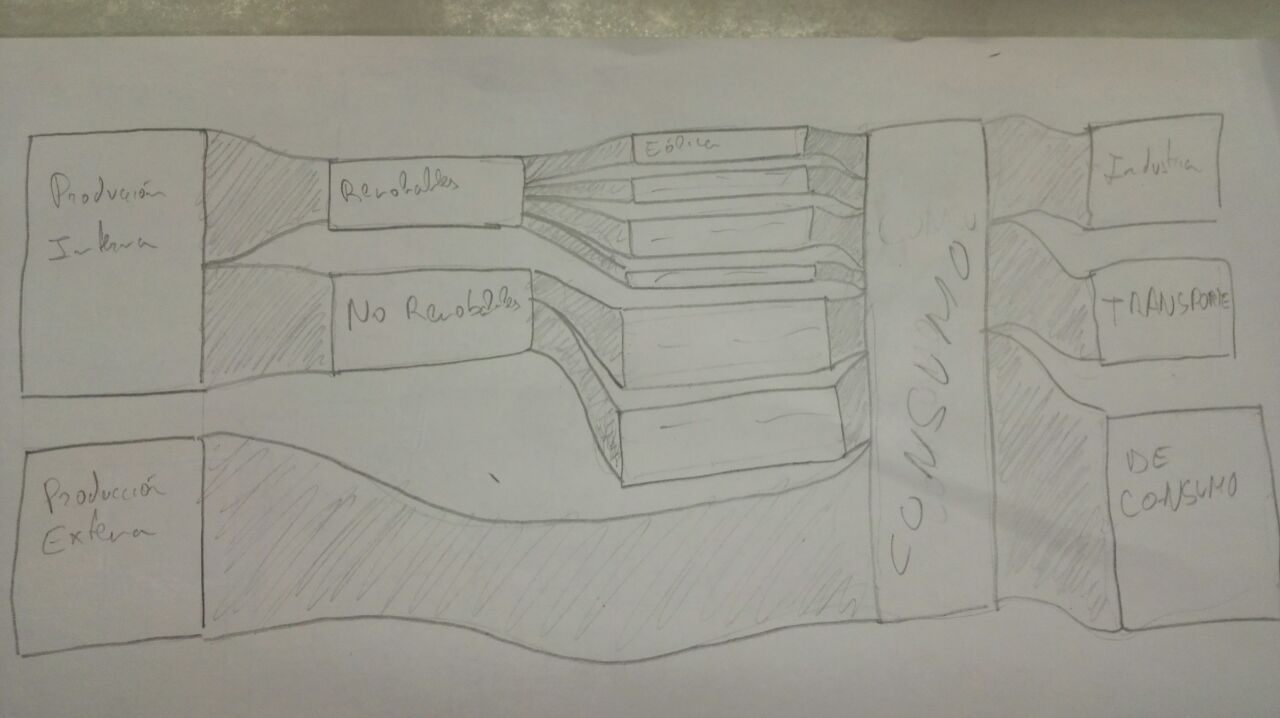
\includegraphics[width=140mm]{../res/sketch-sankey.jpg}
				\caption{Alternativa 2 - Boceto Sankey \label{sketchSankey}}
			\end{figure}
			
			\begin{figure}[H]
				\centering
				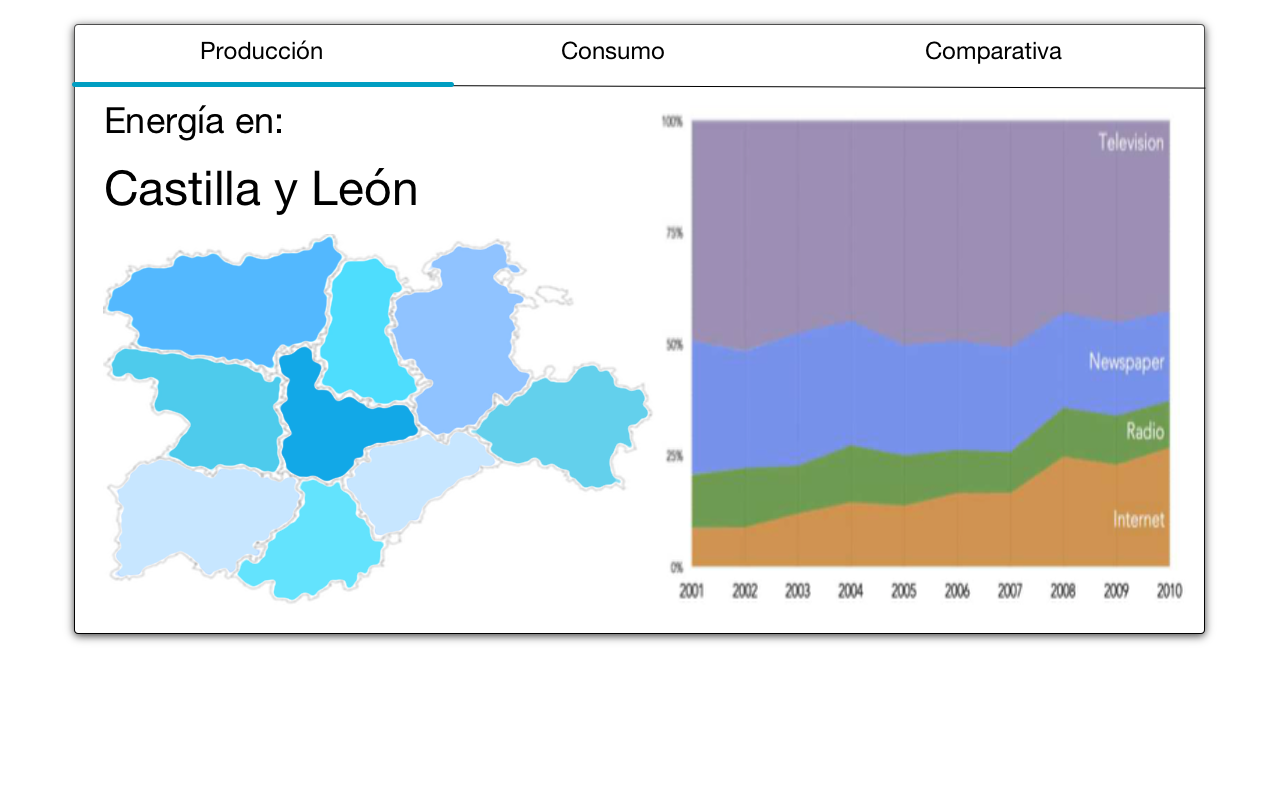
\includegraphics[width=100mm]{../res/design2-1.png}
				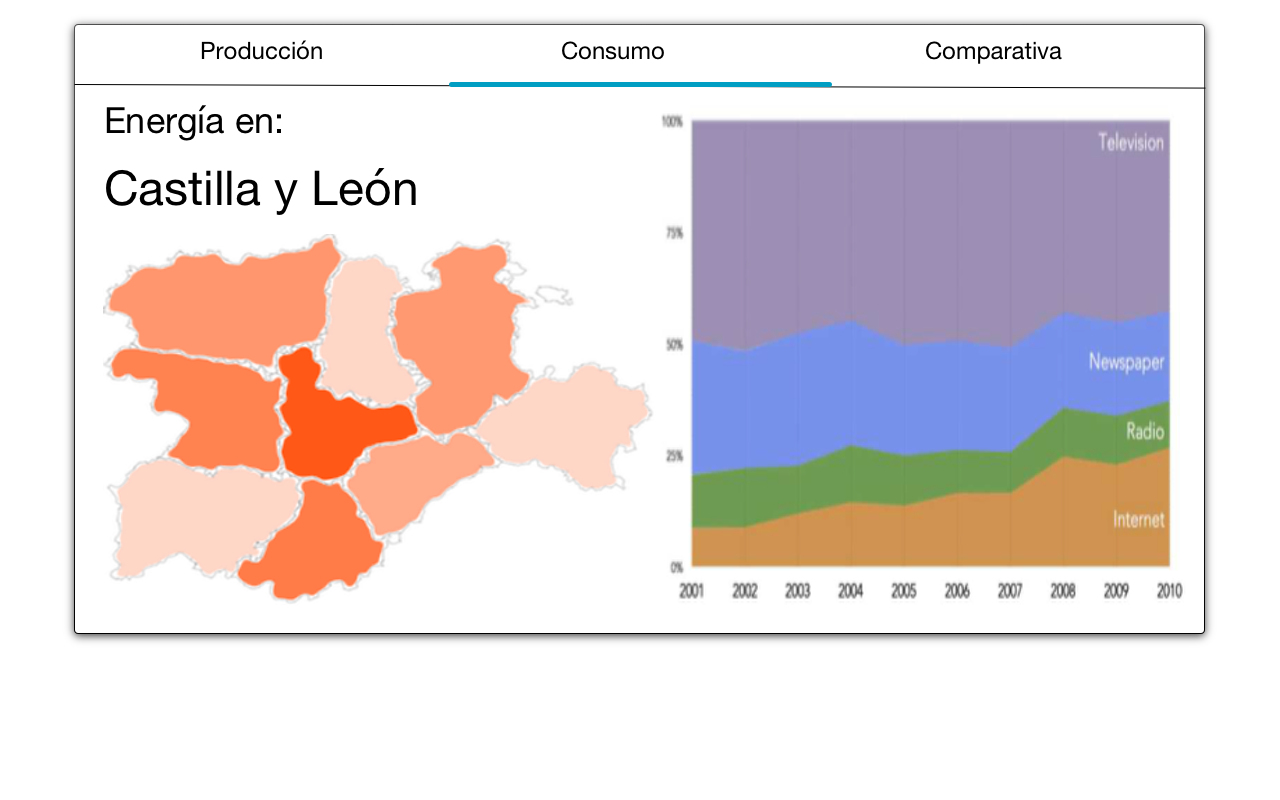
\includegraphics[width=100mm]{../res/design2-2.png}
				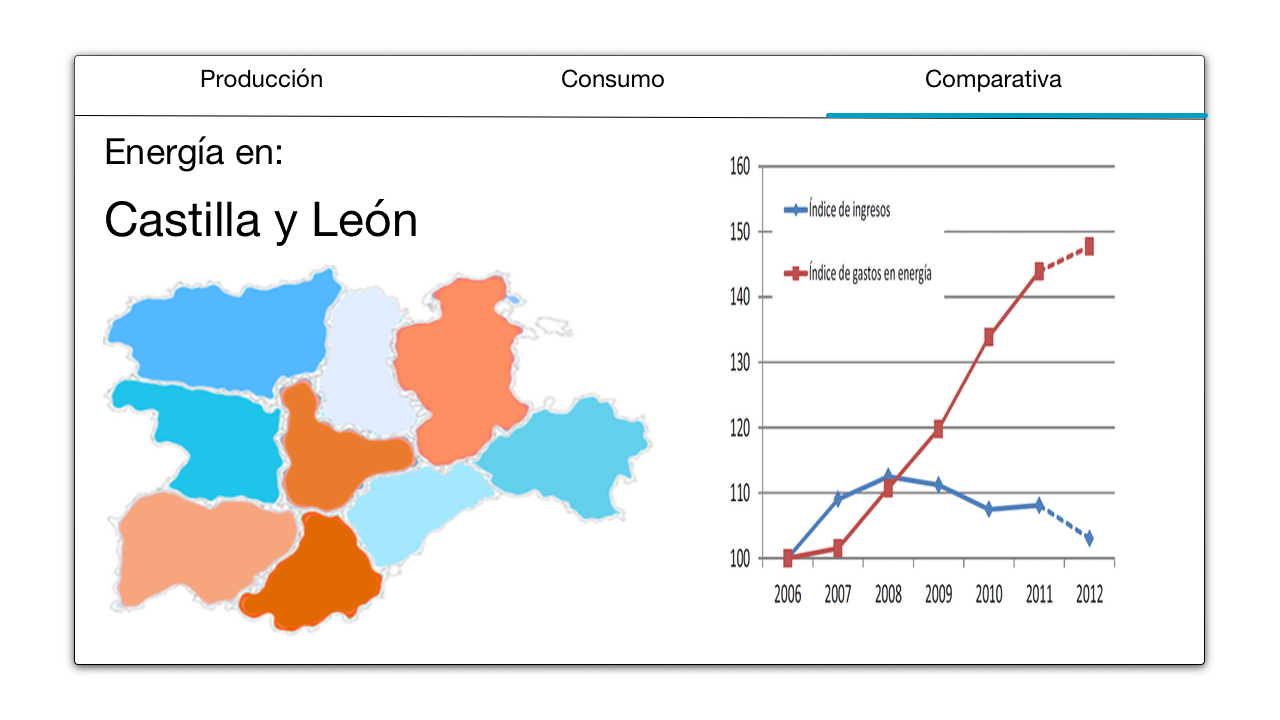
\includegraphics[width=100mm]{../res/design2-3.png}
				\caption{Alternativa 1 - Representación 1 \label{sketch1}}
			\end{figure}
		
			\begin{figure}[H]
				\centering
				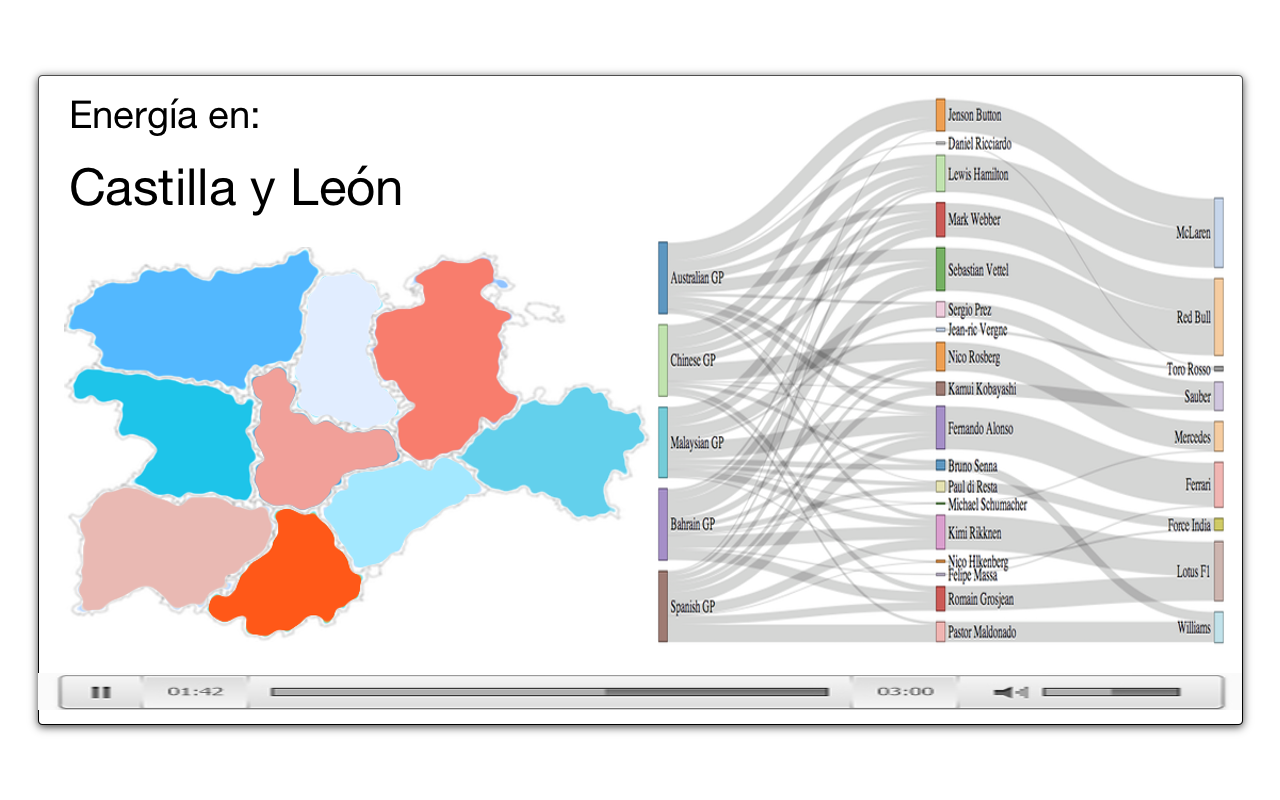
\includegraphics[width=130mm]{../res/design3.png}
				\caption{Alternativa 2 - Representación 1 \label{sketch21}}
			\end{figure}
		
			\begin{figure}[H]
				\centering
				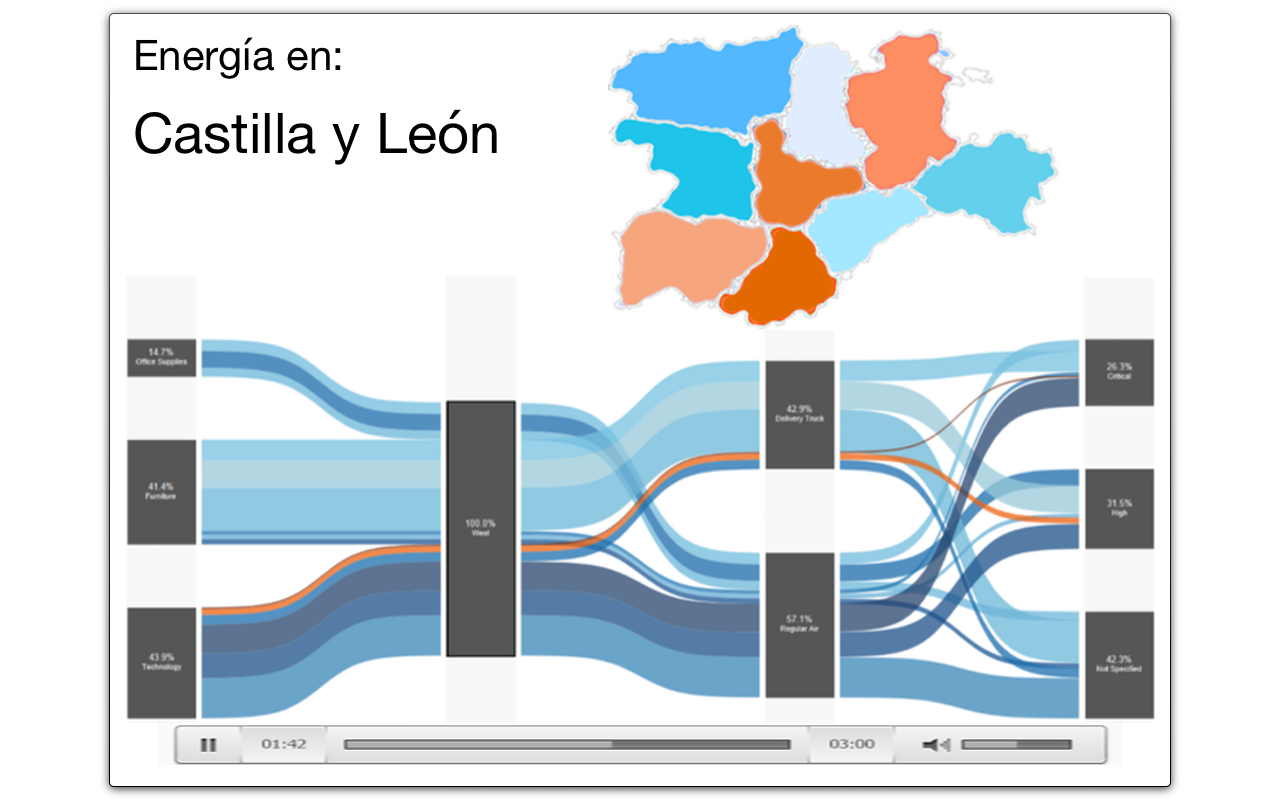
\includegraphics[width=130mm]{../res/design4.png}
				\caption{Alternativa 2 - Representación 2 \label{sketch22}}
			\end{figure}

			\begin{figure}[H]
				\centering
				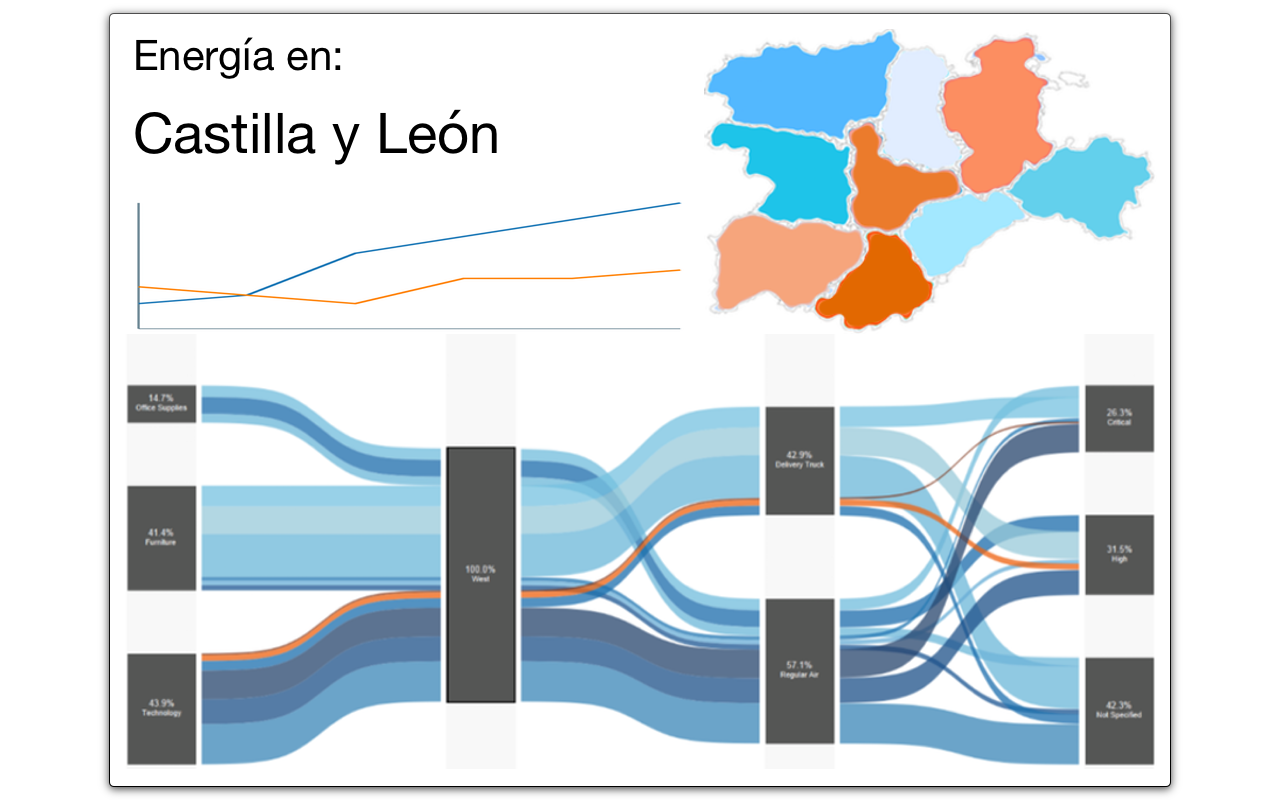
\includegraphics[width=130mm]{../res/design5.png}
				\caption{Alternativa 3  - Representación 1\label{sketch3}}
			\end{figure}
			
	\section{Conclusiones}

		\subsection{Conclusiones}
			
			\paragraph{}
			Tras analizar las dos alternativas expuestas se seleccionó la segunda alternativa, concretamente la segunda representación ya que es la que mejor estética tiene de entre las dos.
			
			\paragraph{}
			Se ha escogido esta alternativa frente a la primera porque permite "de un solo vistazo" conocer el flujo de energía de la comunidad autónoma sacrificando la visión directa del tiempo.



		\subsection{Aspectos a Resaltar}


		\subsection{Cuestiones no tenidas en cuenta}



\end{document}
